% arara: pdflatex: { options: ["--synctex=1"] }
% arara: biber if changed('references.bib')
% arara: pdflatex: { options: ["--synctex=1"] } if changed('expanded.tex')
% arara: pdflatex: { options: ["--synctex=1"] } if changed('expanded.tex')

%%%
 % File: /latex/big-cocluster-paper/expanded.tex
 % Created Date: Tuesday, May 28th 2024
 % Author: Zihan
 % -----
 % Last Modified: Wednesday, 29th May 2024 11:05:20 am
 % Modified By: the developer formerly known as Zihan at <wzh4464@gmail.com>
 % -----
 % HISTORY:
 % Date      		By   	Comments
 % ----------		------	---------------------------------------------------------
%%%

\documentclass[letterpaper, 10 pt, conference]{ieeeconf}  \overrideIEEEmargins                                      

\usepackage{algorithm,algorithmic}
\usepackage{bm}
\usepackage{amsmath}
\usepackage{amssymb}


\usepackage[utf8]{inputenc} \usepackage[T1]{fontenc}    \usepackage{hyperref}       \usepackage{url}            \usepackage{booktabs}       \usepackage{amsfonts}       \usepackage{nicefrac}       \usepackage{microtype}      \usepackage{cleveref}       \usepackage{lipsum}         \usepackage{graphicx}
\usepackage{multirow}       \usepackage[backend=biber,style=ieee]{biblatex}
\bibliography{references}  
\DeclareFieldFormat{url}{}
\DeclareFieldFormat{urldate}{}
\usepackage{doi}
\usepackage{threeparttable}
\usepackage{xcolor}
\usepackage{subcaption}

 

\newtheorem{theorem}{Theorem}

\makeatletter
\def\input@path{{sections/}}
\makeatother

\graphicspath{{images/}}

\title{\LARGE \bf Scalable Co-Clustering for Large-Scale Data through Dynamic Partitioning and Hierarchical Merging}





\author{ 
}




\renewcommand{\cite}[1]{~\autocite{#1}}

\hypersetup{
pdftitle={A template for the arxiv style},
pdfsubject={q-bio.NC, q-bio.QM},
pdfauthor={Zihan Wu},
pdfkeywords={First keyword, Second keyword, More},
}

\begin{document}
\maketitle

\thispagestyle{empty}
\pagestyle{empty}



\begin{abstract}
    Co-clustering simultaneously clusters rows and columns, revealing more fine-grained groups. However, existing co-clustering methods suffer from poor scalability and cannot handle large-scale data. This paper presents a novel and scalable co-clustering method designed to uncover intricate patterns in high-dimensional, large-scale datasets. Specifically, we first propose a large matrix partitioning algorithm that partitions a large matrix into smaller submatrices, enabling parallel co-clustering. This method employs a probabilistic model to optimize the configuration of submatrices, balancing the computational efficiency and depth of analysis.
    Additionally, we propose a hierarchical co-cluster merging algorithm that efficiently identifies and merges co-clusters from these submatrices, enhancing the robustness and reliability of the process. Extensive evaluations validate the effectiveness and efficiency of our method. Experimental results demonstrate a significant reduction in computation time, with an approximate 83\% decrease for dense matrices and up to 30\% for sparse matrices.

\end{abstract}

\section{Introduction}

Artificial Intelligence is a rapidly advancing technology that facilitates complex data analysis, pattern recognition, and decision-making processes. Clustering, a fundamental unsupervised learning technique, groups data points based on shared features, aiding in interpreting complex data structures. However, traditional clustering algorithms \cite{zhang2023AdaptiveGraphConvolution, yuan2023JointNetworkTopology, wu2023EffectiveClusteringStructured} treat all features of data uniformly and solely cluster either rows (samples) or columns (features), as shown in Figure \ref{fig:cluster}. This oversimplified interpretation overlooks critical context-specific relationships within the data, especially when dealing with large, high-dimensional datasets \cite{chen2023FastFlexibleBipartite, zhao2023MultiviewCoclusteringMultisimilarity, kumar2023CoclusteringBasedMethods}.

\textit{Co-clustering} \cite{cheng2000BiclusteringExpressionData, kluger2003SpectralBiclusteringMicroarray, yan2017CoclusteringMultidimensionalBig} is a technique that groups rows (samples) and columns (features) simultaneously, as shown in Figure \ref{fig:cocluster}. It can reveal complex correlations between two different data types and is transformative in scenarios where the relationships between rows and columns are as important as the individual entities themselves. For example, in bioinformatics, co-clustering can identify gene-related patterns leading to biological insights by concurrently analyzing genes and conditions \cite{higham2007SpectralClusteringIts, kluger2003SpectralBiclusteringMicroarray, madeira2004BiclusteringAlgorithmsBiological, zhao2012BiclusteringAnalysisPattern, golchev2015BiclusteringAnalysisGene}. In recommendation systems, co-clustering can discover more fine-grained relationships between users and projects \cite{dhillon2007WeightedGraphCuts, chen2023ParallelNonNegativeMatrix, bouchareb2019ModelBasedCoclustering}. Co-clustering extends traditional clustering methods, enhancing accuracy in pattern detection and broadening the scope of analyses.

\begin{figure}[htbp]
    \centering
    \begin{subfigure}[b]{0.22\textwidth}
        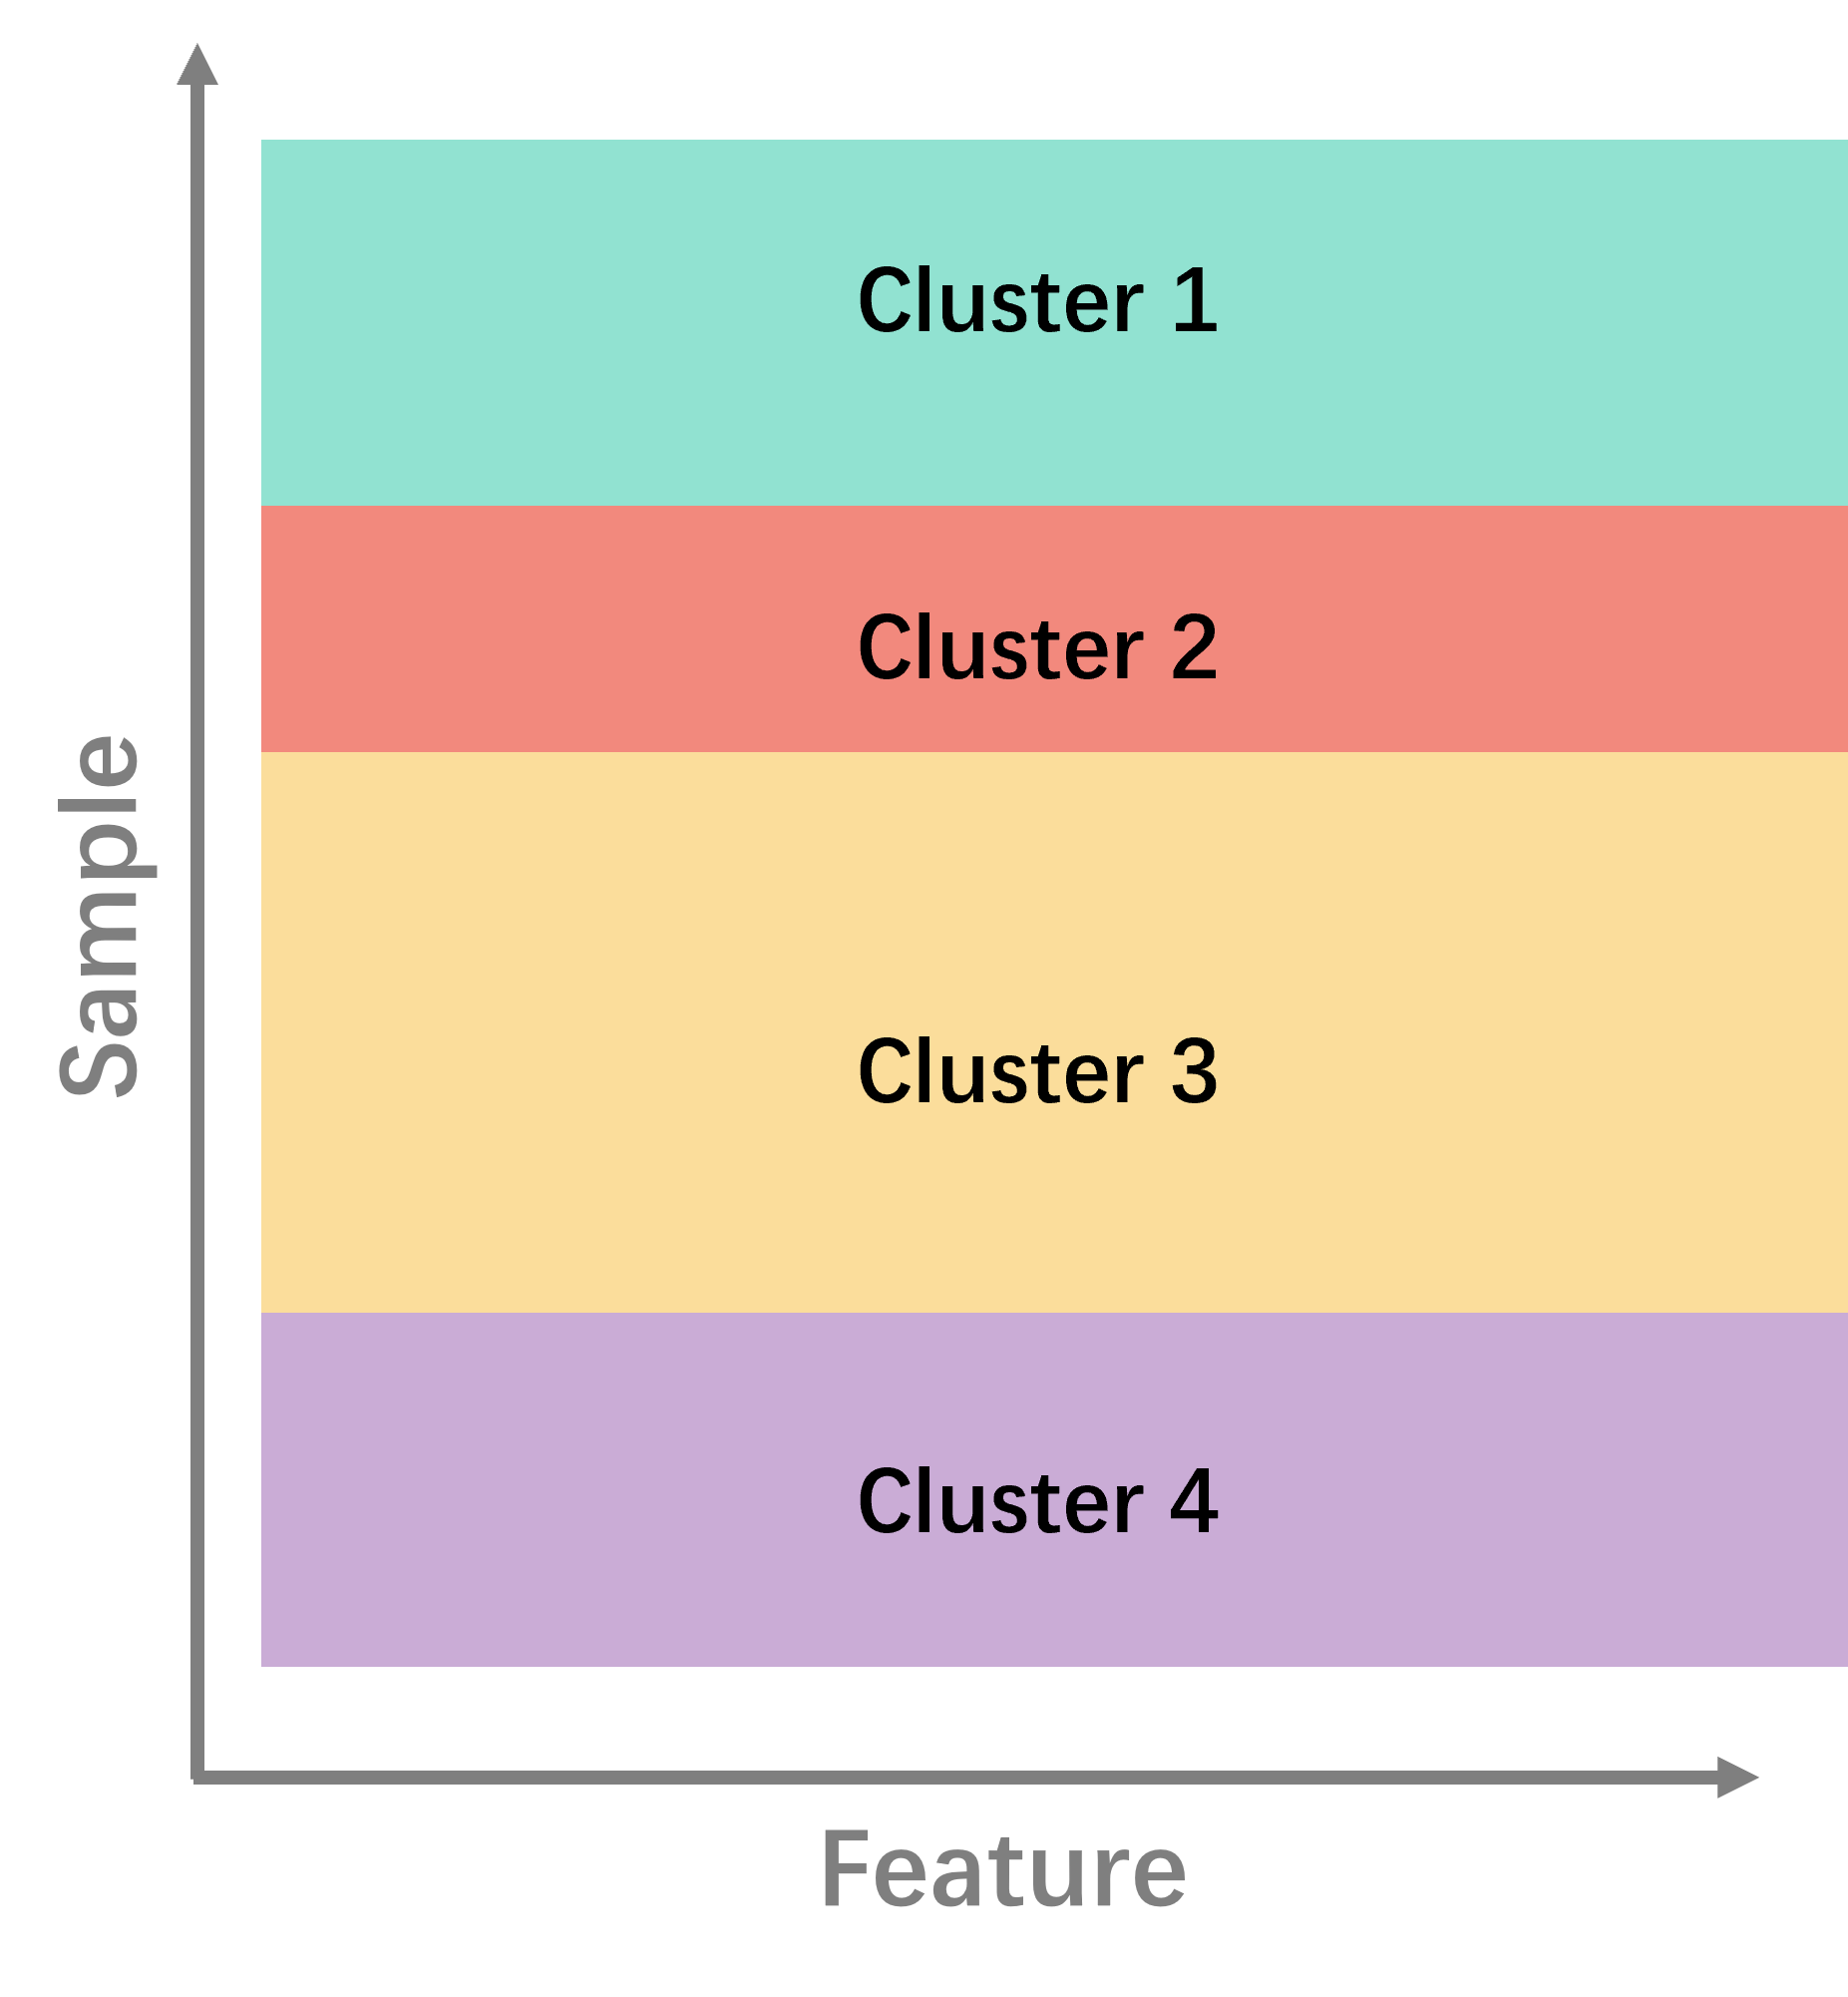
\includegraphics[width=\linewidth]{cluster.png}
        \caption{Clustering}
        \label{fig:cluster}
    \end{subfigure}
    \hfill
    \begin{subfigure}[b]{0.22\textwidth}
        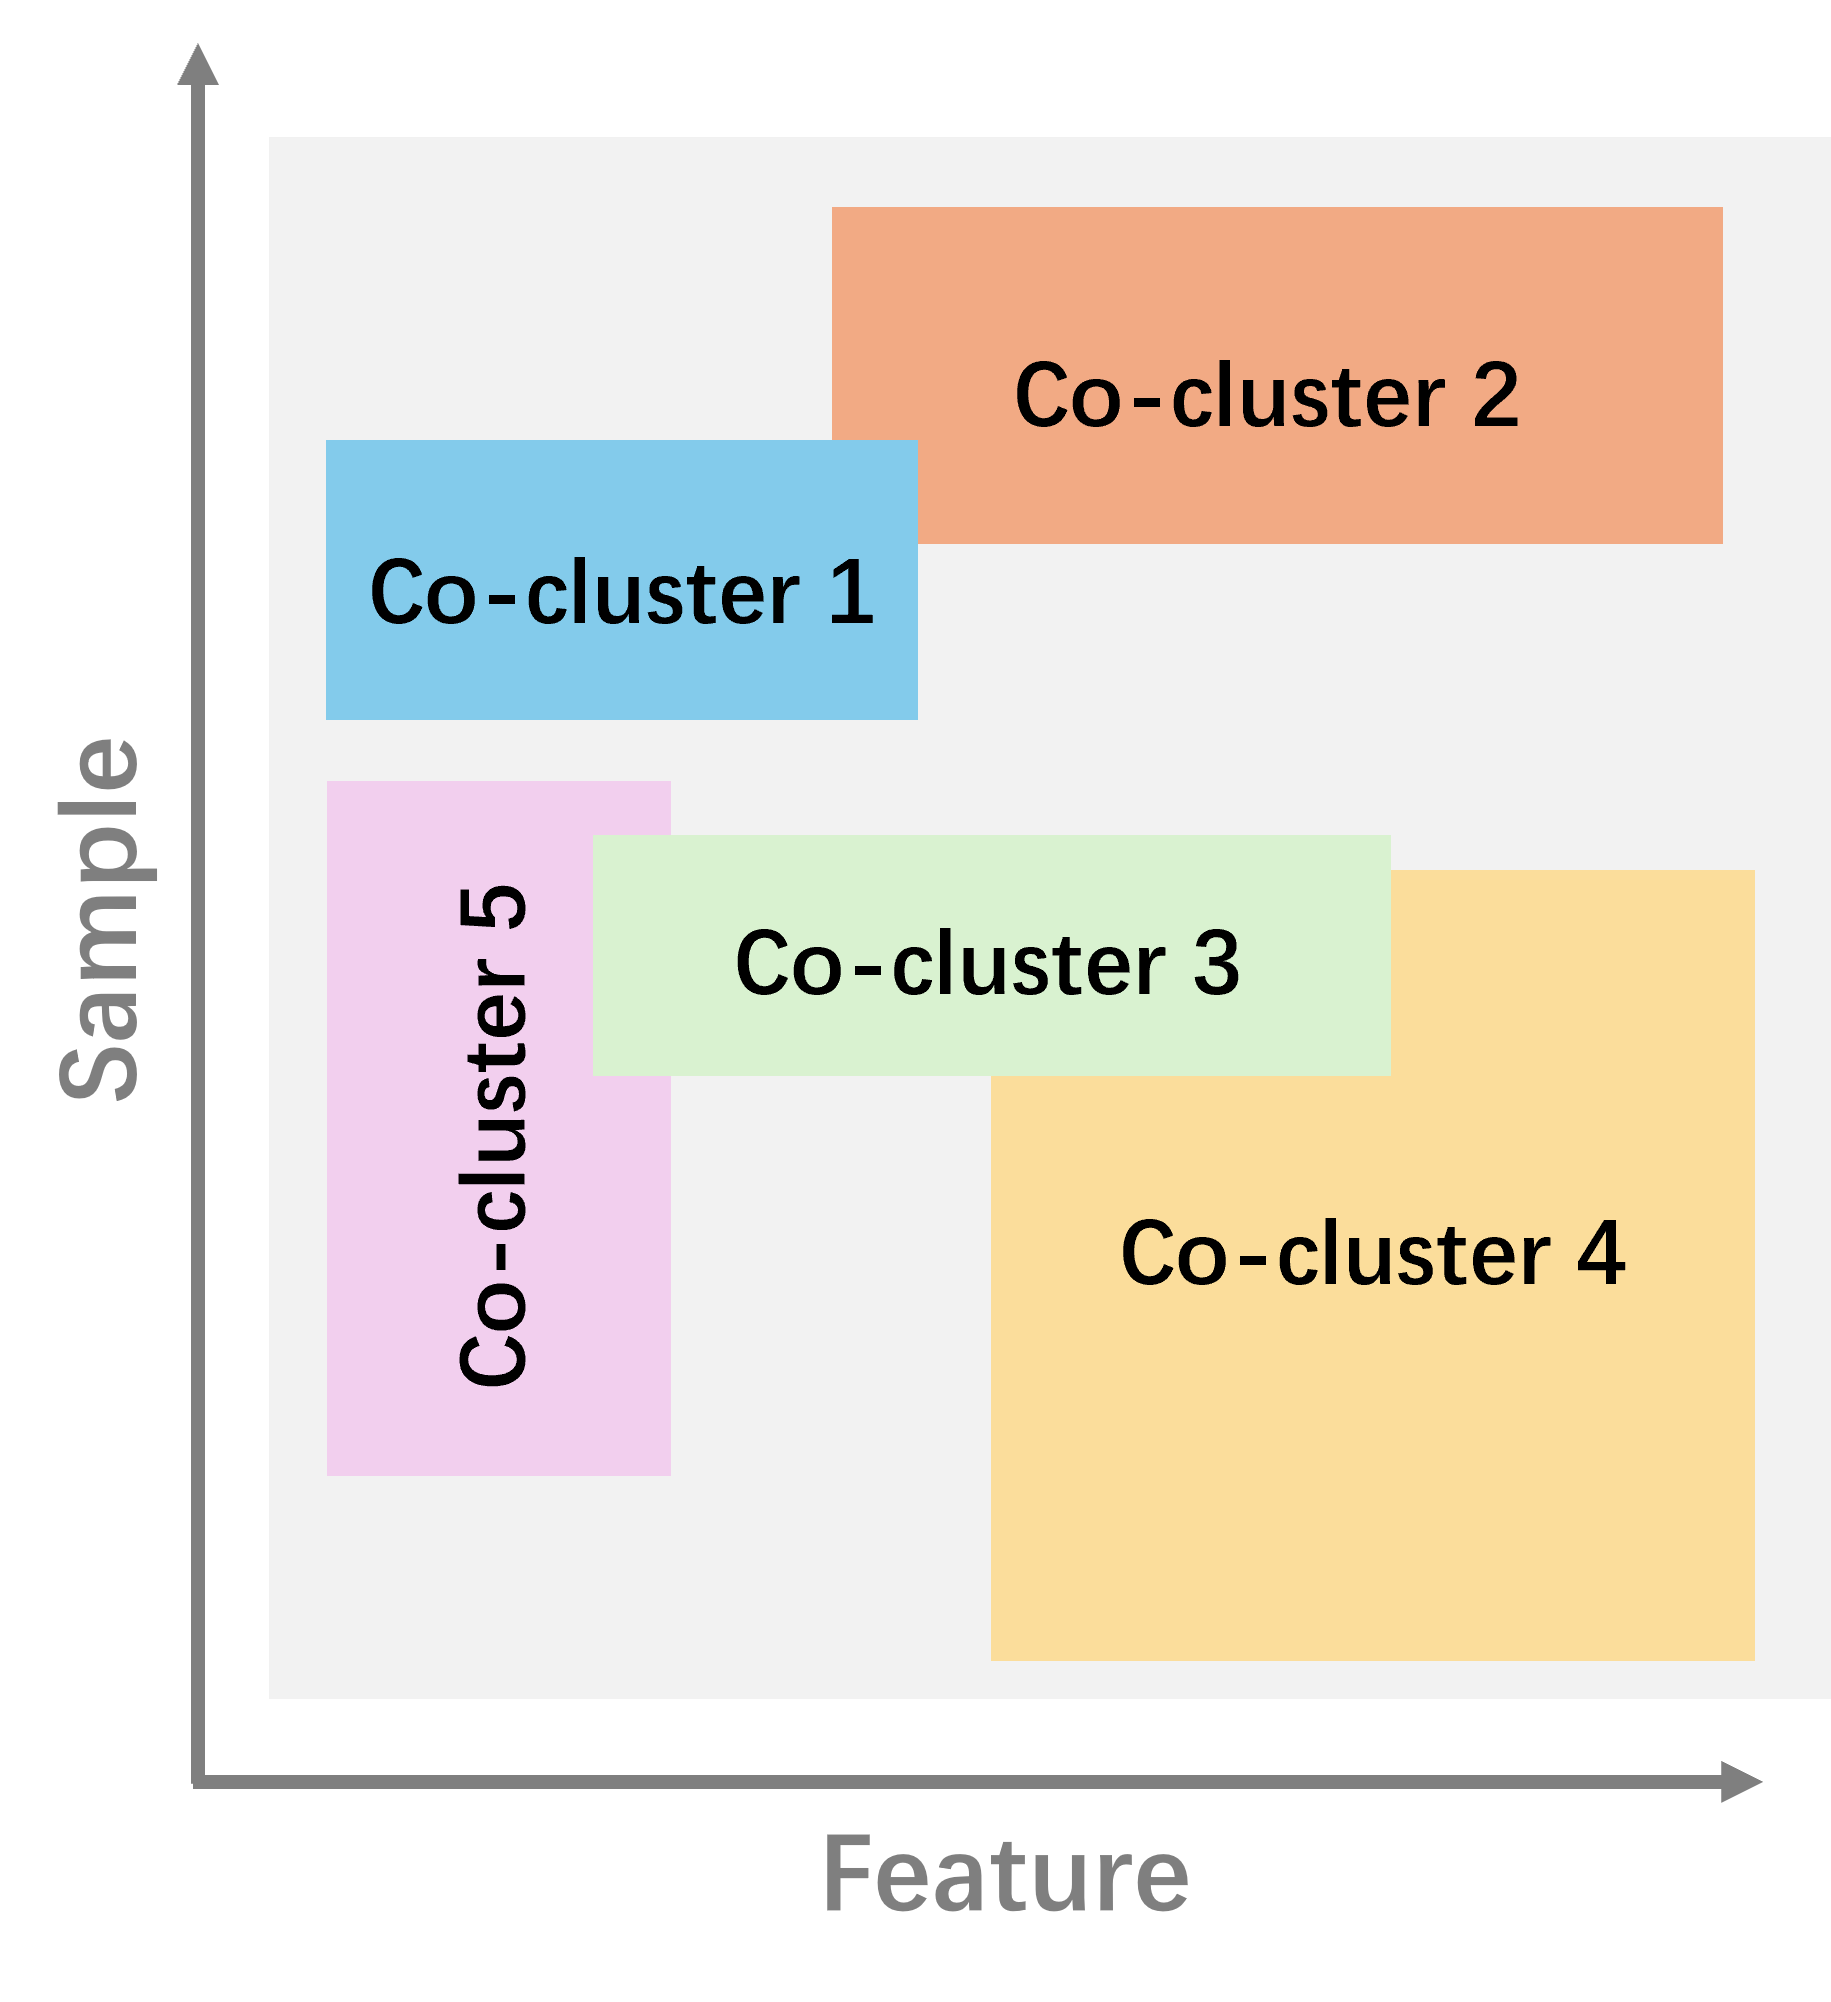
\includegraphics[width=\linewidth]{coc.png}
        \caption{Co-clustering}
        \label{fig:cocluster}
    \end{subfigure}
    \caption{An illustration of the differences between (a) Clustering and (b) Co-clustering.}
    \label{fig:cocomparison}
\end{figure}

Despite its potential, scaling co-clustering to large datasets poses significant challenges:
\begin{enumerate}
    \item \textbf{High Computational Complexity}: Co-clustering analyzes relationships both within and across the rows and columns of a dataset simultaneously. This dual-focus analysis requires evaluating a vast number of potential relationships, particularly as the dimensions of the data increase. The complexity can grow exponentially with the size of the data because the algorithm must process every possible combination of rows and columns to identify meaningful clusters.
    \item \textbf{Significant Communication Overhead}: Even when methods such as data partitioning are used to handle large-scale data, each partition may independently analyze a subset of the data. However, to optimize the clustering results globally, these partitions need to exchange intermediate results frequently. This requirement is inherent to iterative optimization techniques used in co-clustering, where each iteration aims to refine the clusters based on new data insights, necessitating continuous updates across the network. Such extensive communication can become a bottleneck, significantly slowing down the overall processing speed.
    \item \textbf{Dependency on Sparse Matrices}: Many traditional co-clustering algorithms are designed to perform best with sparse matrices, where most elements are zero. However, in many real-world applications, data matrices are often dense, meaning most elements are non-zero. Such scenarios present a significant challenge for standard co-clustering algorithms, as they must handle a larger volume of data without the computational shortcuts available with sparse matrices.
\end{enumerate}

To address the inherent challenges associated with existing co-clustering methods, we propose a novel and scalable co-clustering method designed for large-scale datasets. First, we propose a large matrix partitioning algorithm that divides the original data matrix into smaller submatrices. This partitioning facilitates parallel processing of co-clustering tasks across submatrices, significantly reducing both processing time and computational and storage demands for each processing unit. We also design a probabilistic model to determine the optimal number and configuration of these submatrices to ensure comprehensive data coverage. Second, we develop a hierarchical co-cluster merging algorithm that iteratively combines the co-clusters from these submatrices. This process enhances the accuracy and reliability of the final co-clustering results and ensures robust and consistent clustering performance, particularly addressing issues of heterogeneity and model uncertainty.

The contributions of this paper are summarized as follows:
\begin{enumerate}
    \item \textbf{Large Matrix Partitioning Algorithm:}
          We propose a novel matrix partitioning algorithm that enables parallel co-clustering by dividing a large matrix into optimally configured submatrices. This design is supported by a probabilistic model that calculates the optimal number and order of submatrices, balancing computational efficiency with the detection of relevant co-clusters.
    \item \textbf{Hierarchical Co-cluster Merging Algorithm:}
          We design a hierarchical co-cluster merging algorithm that combines co-clusters from submatrices, ensuring the completion of the co-clustering process within a pre-fixed number of iterations. This algorithm significantly enhances the robustness and reliability of the co-clustering process, effectively addressing model uncertainty.
    \item \textbf{Experiment valuation:}
          We evaluate the effectiveness and efficiency of our method across a wide range of scenarios with large, complex data. Experimental results show an approximate 83\% decrease for dense matrices and up to 30\% for sparse matrices.
\end{enumerate}

The rest of this paper is organized as follows. Section \ref{sec:related_work} reviews related works. Section \ref{sec:formula} introduces the mathematical formulation and the goal of this paper. Then, Section \ref{sec:method} describes our scalable co-clustering method. Section \ref{sec:experiment} presents experiments and results, validating the efficacy of our method. Section \ref{sec:conclude} concludes the paper, summarizing our findings and discussing potential avenues for future research in this domain.


\section{Related work}
\label{sec:related_work}
\subsection{Co-clustering Methods}
Co-clustering methods employing Singular Value Decomposition (SVD) can be broadly categorized into graph-based and matrix factorization-based approaches
\cite{dhillon2001CoclusteringDocumentsWords}. A prominent example of graph-based co-clustering is the Flexible Bipartite Graph Co-clustering (FBGPC) \cite{chen2023FastFlexibleBipartitea}, which directly applies a flexible bipartite graph model to the original data. In contrast, Non-negative Matrix Tri-Factorization (NMTF) represents a leading matrix factorization-based method that decomposes data into multiple matrices to independently cluster samples and features, subsequently discovering the relationships between them \cite{long2005CoclusteringBlockValue}. Our method is orthogonal to NMTF, allowing for potential integration to enhance co-clustering efficiency.

Another innovative method, Deep Co-Clustering (DeepCC), integrates deep autoencoders with Gaussian Mixture Models to improve data clustering \cite{dongkuanxu2019DeepCoClustering}. Despite its advancements, DeepCC struggles with computational efficiency, particularly with diverse data types and iterative processes dependent on data sparsity.

\subsection{Parallelizing Co-clustering}

Parallel co-clustering methods have emerged as a vital solution to the challenges of processing big data. The CoClusterD framework by Cheng \textit{et al.} \cite{cheng2015CoClusterDDistributedFramework} utilizes an Alternating Minimization Co-clustering (AMCC) algorithm with sequential updates in a distributed environment. However, this method faces challenges with guaranteed convergence, leading to potential inefficiencies.

While matrix factorization techniques have shown promise for co-clustering large datasets, scaling to massive high-dimensional data remains an open challenge. Chen \textit{et al.}\cite{chen2023ParallelNonNegativeMatrix} proposed a parallel non-negative matrix tri-factorization method that distributes computation across multiple nodes to accelerate factorizations. However, even these advanced methods encounter difficulties with extremely large datasets.

Our proposed method adopts a divide-and-conquer strategy, partitioning the input matrix into smaller submatrices, which are then co-clustered in parallel. This technique reduces the complexity imposed by high dimensionality and combines the results to form the final co-clusters. This novel approach addresses the computational challenges and introduces a scalable solution for big data.

\section{Mathematical Formulation and Problem Statement}\label{sec:formula}
\subsection{Mathematical Formulation of Co-clustering}
Co-clustering is a method designed to simultaneously group a set of rows and columns in a data matrix $\mathbf{A} \in \mathbb{R}^{M \times N}$, where $M$ denotes the number of features or variables and $N$ denotes the number of samples or objects. Each element $a_{ij}$ in the matrix at the $(i, j)$-th position represents the relationship or measurement between the $i$-th feature and the $j$-th object. The primary goal of co-clustering is to identify subsets of rows ($I$) and columns ($J$) into homogenous submatrices, $\mathbf{A}_{I, J}$, that exhibit distinctive patterns or uniform characteristics, thus forming coherent co-clusters. The objective is to partition $\mathbf{A}$ into $k$ row clusters and $d$ column clusters, resulting in $k \times d$ distinct co-clusters.

When rows and columns are optimally reordered, $\mathbf{A}$ can be visualized as a block-diagonal matrix, where each block represents a co-cluster with higher similarity within than between blocks. We define the row and column label sets as \( u \in \{1,\dots,k\}^M \) and \( v \in \{1,\dots,d\}^N \), respectively. Indicator matrices \( R \in \mathbb{R}^{M \times k} \) and \( C \in \mathbb{R}^{N \times d} \) are used to assign rows and columns to clusters, with the constraints \( \sum_k R_{i,k} = 1 \) and \( \sum_d C_{j,d} = 1 \), ensuring each row and column is assigned to exactly one cluster.

\subsection{Problem Statement}
This paper aims to develop a method that efficiently and accurately identifies co-clusters $\mathbf{A}_{I, J}$ within a matrix $\mathbf{A}$ representing large datasets. These co-clusters should exhibit specific structural patterns such as uniformity across elements, consistency along rows or columns, or patterns demonstrating additive or multiplicative coherence. Properly identifying and categorizing these patterns is crucial for understanding the complex data structures inherent in large datasets. This method is intended to improve the detection capabilities of co-clustering, enhancing both the efficiency and precision necessary for handling large-scale data challenges.


\section{The Scalable Co-clustering Method}
\label{sec:method}
\subsection{Overview}

\begin{figure*}[htbp]
    \centering
    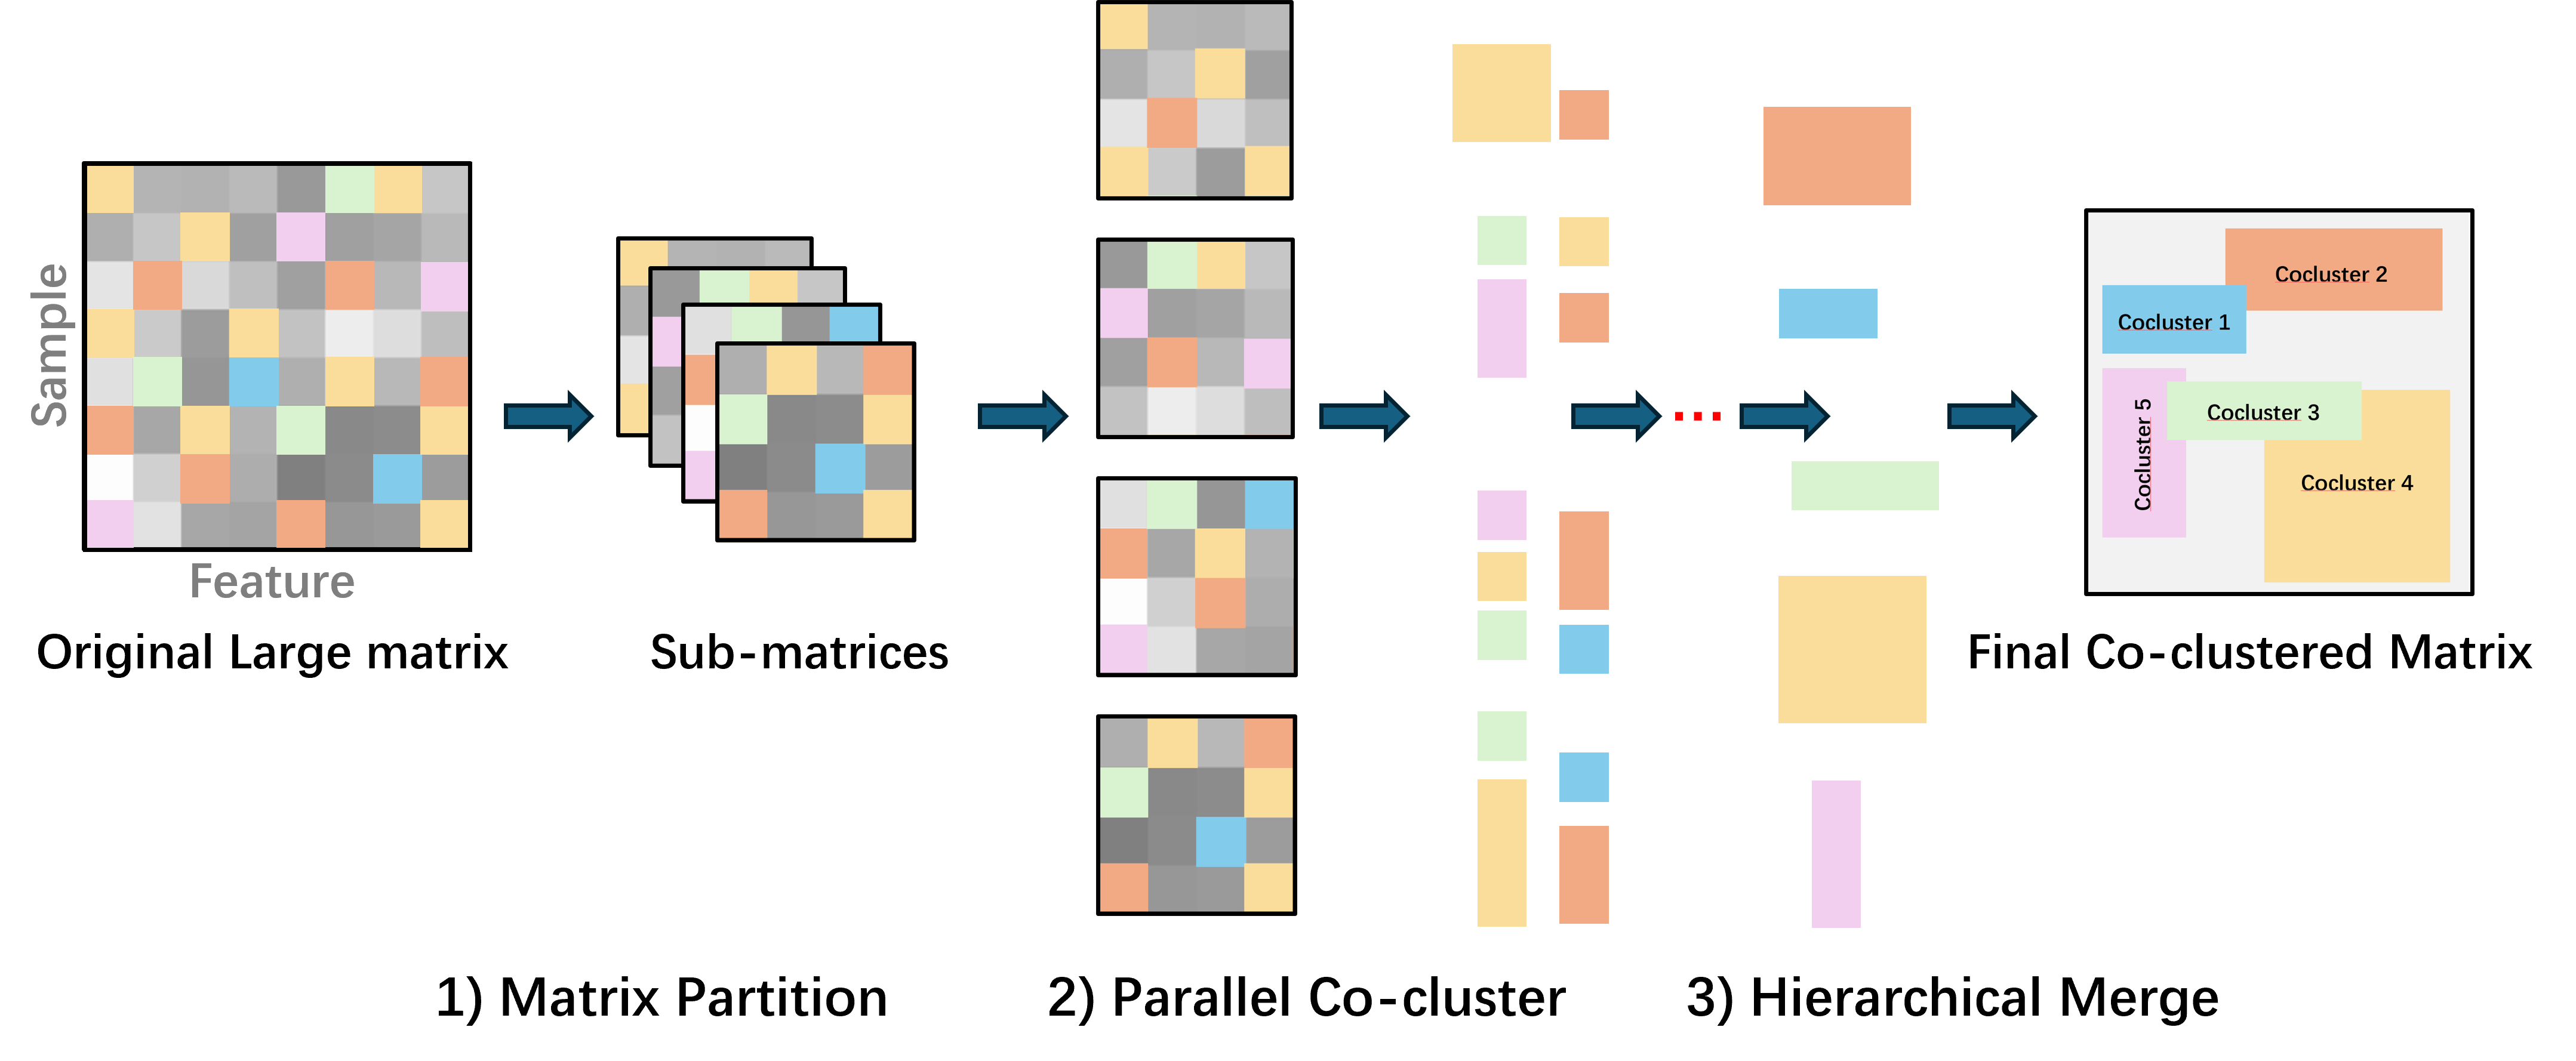
\includegraphics[width=0.8\linewidth]{workflow.png}
    \caption{Workflow of our proposed scalable co-clustering method for large matrices.}
    \label{fig:workflow}
\end{figure*}
This paper presents a novel and scalable co-cluster method specifically designed for large matrices, as shown in \Cref{fig:workflow}. This method applies a probabilistic model-based optimal partitioning algorithm, which not only predicts the ideal number and sequence of partitions for maximizing computational efficiency but also ensures the effectiveness of the co-clustering process.

Our method involves partitioning large matrices into smaller, manageable submatrices. This strategic partitioning is meticulously guided by our algorithm to facilitate parallel processing. By transforming the computationally intensive task of co-clustering a large matrix into smaller, parallel tasks, our approach significantly reduces computational overhead and enhances scalability.

Following the partitioning, each submatrix undergoes a co-clustering process. This is implemented via the application of Singular Value Decomposition (SVD) and $k$-means clustering on the resulting singular vectors. This pivotal step ensures the adaptability of our method, allowing our algorithm to tailor its approach to the unique characteristics of each submatrix, thus optimizing clustering results.

Furthermore, our method integrates a novel hierarchical merging strategy that combines the co-clustering results from all submatrices. This integration provides more fine-grained insight into each submatrix and enhances the overall accuracy and reliability of the co-clustering results. Our method, validated and optimized through a comprehensive process, showed efficiency in handling large-scale datasets that were never reached before.


\subsection{Large Matrix Partitioning}
The primary challenge in co-clustering large matrices is the risk of losing meaningful co-cluster relationships when the matrix is partitioned into smaller submatrices. To address this, we introduce an optimal partitioning algorithm underpinned by a probabilistic model. This model is meticulously designed to navigate the complexities of partitioning, ensuring that the integrity of co-clusters is maintained even as the matrix is divided. The objective of this algorithm is twofold: to determine the optimal partitioning strategy that minimizes the risk of fragmenting significant co-clusters and to define the appropriate number of repartitioning iterations needed to achieve a desired success rate of co-cluster identification.

\subsubsection{Partitioning and Repartitioning Strategy based on the Probabilistic Model}
Our probabilistic model serves as the cornerstone of the partitioning algorithm. It evaluates potential partitioning schemes based on their ability to preserve meaningful co-cluster structures within smaller submatrices. The model operates under the premise that each atom-co-cluster (the smallest identifiable co-cluster within a submatrix) can be identified with a probability $p$. This probabilistic model allows us to estimate the likelihood of successfully identifying all relevant co-clusters across the partitioned submatrices.

In the scenario where the matrix $A$ is partitioned into $m \times n$ blocks, each block has size $\phi_i \times \psi_j$, that is, $M=\sum_{i=1}^m \phi_i$ and $N=\sum_{j=1}^n \psi_j$, the joint probability of $M_{(i,j)}^{(k)}$ and $N_{(i,j)}^{(k)}$ are
\begin{align*}
    P(M_{(i,j)}^{(k)} & < T_m, N_{(i,j)}^{(k)} < T_n)                               \\ & = \sum_{\alpha=1}^{T_m-1} \sum_{\beta=1}^{T_n-1} P(M_{(i,j)}^{(k)} = \alpha) P(N_{(i,j)}^{(k)} = \beta) \\
                      & \le \exp[-2 (s_i^{(k)})^2 \phi_i + -2 (t_j^{(k)})^2 \psi_j]
\end{align*}
where $s_i^{(k)}$ and $t_j^{(k)}$ are the minimum row and column sizes of co-cluster $C_k$ in block $B_{(i,j)}$, the size of the co-cluster $C_k$ is $M^{(k)} \times N^{(k)}$, and $M^{(k)}$ and $N^{(k)}$ are the row and column sizes of co-cluster $C_k$, respectively.



Thus, the probability of identifying all co-clusters is given by

\begin{align}
    P(\omega_k) & \le \exp \left\{ -2 [\phi m (s^{(k)})^2 + \psi n (t^{(k)})^2] \right\},
\end{align}
and
\begin{align}
    P & = 1 - P(\omega_k)^{T_p}                                                                                                       \\
      & \ge 1 - \exp \left\{ -2 T_p [\phi m (s^{(k)})^2 + \psi n (t^{(k)})^2] \right\} \label{eq:prob_of_identifying_all_co_clusters}
\end{align}
where $P(\omega_k)$ is the probability of the failure of identifying co-cluster $C_k$, $T_p$ is the number of sampling times, $\phi$ and $\psi$ are the row and column block sizes, and $s^{(k)}$ and $t^{(k)}$ are the minimum row and column sizes of co-cluster $C_k$.


\Cref{eq:prob_of_identifying_all_co_clusters} is central to our algorithm for partitioning large matrices for co-clustering, providing a probabilistic model that informs and optimizes our partitioning strategy to preserve co-cluster integrity. It mathematically quantifies the likelihood of identifying all relevant co-clusters within partitioned blocks, guiding us to mitigate risks associated with partitioning that might fragment vital co-cluster relationships.

Based on \Cref{eq:prob_of_identifying_all_co_clusters}, we can establish a constraint between the repartitioning time $Tr$ and the partition solution $Part$, ensuring that the partitioning strategy adheres to a predetermined tolerance success rate, thereby minimizing the risk of co-cluster fragmentation. The constraints are discussed in appendix due to space limitations.

\subsubsection{Optimization and Computational Efficiency}
Optimizing the partitioning process for computational efficiency is paramount in both academic and industrial applications, where running time often serves as the primary bottleneck. Thanks to the flexible framework established by our probabilistic model and the constraints derived in Theorem 1, our optimization strategy can be tailored to address the most critical needs of a given context. In this case, we focus on minimizing the running time without compromising the integrity and success rate of co-cluster identification.


Our approach to optimization leverages the probabilistic model to assess various partitioning configurations, balancing the trade-off between computational resource allocation and the need to adhere to theoretical success thresholds. By systematically evaluating the impact of different partitioning schemes on running time, we can identify strategies that not only meet our co-clustering success criteria but also optimize the use of computational resources.

To ensure that our optimization does not sacrifice the quality of co-cluster identification for the sake of efficiency, we introduce a secondary theorem that outlines the conditions under which optimization can be achieved without compromising the success rate of co-cluster discovery. This theorem provides a mathematical basis for optimizing the partitioning algorithm in a manner that maintains a balance between computational efficiency and the fidelity of co-cluster identification.


Under the constraint of maintaining a predetermined success rate $P$ for co-cluster identification, the optimization of the partitioning algorithm with respect to running time must satisfy the following condition:
\begin{align*}
    T_p = \text{argmin}_{T_p} \{
    1 & - \exp \{ -2 T_p [\phi m (s^{(k)})^2         \\
      & + n (t^{(k)})^2] \} \ge P_{\text{thresh}} \}
\end{align*}


This condition delineates the parameters within which the partitioning strategy can be optimized for speed without detracting from the algorithm's ability to accurately identify co-clusters. By adhering to this theorem, we ensure that our optimization efforts align with the overarching goal of preserving the integrity and effectiveness of co-cluster discovery. This balance is crucial for developing a partitioning algorithm that is not only fast and efficient but also robust and reliable across various data sets and co-clustering challenges.

\subsection{Co-clustering on Small Submatrices}


\subsubsection{Atom-co-clustering Algorithm}
Our framework, which encompasses both partitioning and ensembling, offers remarkable flexibility, allowing it to be compatible with a wide range of atom-co-clustering methods. For the sake of making this paper comprehensive and self-contained, we provide an introduction to the atom-co-cluster method herein. The only requirement for an atom-co-clustering method to be compatible with our framework is that it must be able to identify co-clusters under a given criterion with a probability $p$, or more relaxed conditions, has a lower bound estimate of the probability of identifying co-clusters equipped with a validation mechanism.

\subsubsection{Graph-based Spectral Co-clustering Algorithm}

Spectral co-clustering (SCC) stands as one of the most prevalent methods in the realm of co-clustering today\cite{vonluxburg2007TutorialSpectralClustering}, primarily due to its adeptness in unraveling the complexities of high-dimensional data. At its core, this method harnesses the power of spectral clustering principles, focusing on the utilization of a graph's Laplacian matrix eigenvectors for effectively partitioning data into distinct clusters. This approach is exceptionally beneficial for analyzing data that naturally forms a bipartite graph structure, including applications in text-document analysis, social network modeling, and gene expression studies.


\paragraph{Graph Construction in Co-clustering Expanded}

SCC begins with constructing a bipartite graph $G=(U,V,E)$. Here, $U$ and $V$, both as vertex sets, symbolize the sets corresponding to the rows and columns of the data matrix, respectively. The edges $E$ of this graph are assigned weights reflecting the relationships between rows and columns. Consequently, the graph's weighted adjacency matrix $W$ is defined as:

$$ W = \begin{bmatrix} 0 & A \\ A^T & 0 \end{bmatrix}, $$
where $A$ denotes the data matrix, also called adjacency matrix in the graph context.
Through this representation, the challenge of co-clustering is reformulated into a graph partitioning task, aiming to segregate the graph into distinct clusters based on the interrelations between the data matrix's rows and columns.

\paragraph{Laplacian Matrix}

The graph's Laplacian matrix $L$ is computed as $L=D-W$, with $D$ being the graph's degree matrix—a diagonal matrix whose entries equal the sum of the weights of the edges incident to each node. The Laplacian matrix plays a crucial role in identifying the graph's cluster structure. It does so by facilitating the calculation of eigenvectors associated with its smallest positive eigenvalues, which in turn, guide the partitioning of the graph into clusters.

\paragraph{Graph Partitioning and Singular Value Decomposition}
Theorem 4 in \cite{dhillon2001CoclusteringDocumentsWords} states that the eigenvector corresponding to the second smallest eigenvalue of the following eigenvalue problem gives the generalized partition vectors for the graph:

\begin{equation}
    L \mathbf{v} = \lambda D \mathbf{v}
    \label{eq:eigenvalue_problem}
\end{equation}

And according to Section 4 of \cite{dhillon2001CoclusteringDocumentsWords}, the singular value decomposition of the normalized matrix $A_n = D^{-1/2} A D^{-1/2}$
$$A_n = U \Sigma V^T$$
gives the solution to \Cref{eq:eigenvalue_problem}. To be more specific, the singular vectors corresponding to the second largest singular value of $A_n$ is the eigenvector corresponding to the second smallest eigenvalue of \Cref{eq:eigenvalue_problem}.

The above discussion is under the assumption that the graph has only one connected component. In a more general setting, $\mathbf{u_2}, \mathbf{u_3}, \ldots, \mathbf{u_{l+1}}$ and $\mathbf{v_2}, \mathbf{v_3}, \ldots, \mathbf{v_{l+1}}$ reveal the $k$-modal information of the graph, where $\mathbf{u_k}$ and $\mathbf{v_k}$ are the $k$-th left and right singular vectors of $A_n$, respectively.
And for the last step,
$$ Z = \begin{bmatrix} D_1^{-1/2} \hat{U} \\ D_2^{-1/2} \hat{V} \end{bmatrix} $$
is stacked where $\hat{U} = [\mathbf{u_2}; \mathbf{u_3}; \ldots; \mathbf{u_{l+1}}]$ and $\hat{V} = [\mathbf{v_2}; \mathbf{v_3}; \ldots; \mathbf{v_{l+1}}]$. The approximation to the graph partitioning optimization problem is then solved by applying a $k$-means algorithm to the rows of $Z$. More details can be found in \cite{dhillon2001CoclusteringDocumentsWords}.

\subsection{Hierarchical Co-cluster Merging}


Hierarchical co-cluster merging is a novel approach that combines the results of co-clustering on submatrices to produce a final co-clustered result.
The merging method is designed to enhance the accuracy and robustness of the co-clustering outcome by leveraging the design of the partitioning algorithm. The hierarchical merging process iteratively combines the co-clusters from each submatrix, ensuring that the final co-clustered result is comprehensive and consistent across all submatrices. This iterative merging process is crucial for addressing issues of heterogeneity and model uncertainty, ensuring that the final co-clustering results are reliable and robust.

\subsection{Algorithmic Description}
Our proposed  Optimal Matrix Partition and Hierarchical Co-cluster Merging Method is outlined in Algorithm \ref{alg:method}. The algorithm
is an advanced algorithm designed for efficient co-clustering of large data matrices. The algorithm begins by initializing a block set based on predetermined block sizes. For each co-cluster in the given set, the algorithm calculates specific values $s^{(k)}$ and $t^{(k)}$, which are then used to determine the probability $P(\omega_k)$ of each co-cluster. If this probability falls below a predefined threshold $P_{\text{thresh}}$, the algorithm partitions the data matrix $A$ into blocks $B$ and performs co-clustering on these blocks. This step is crucial for managing large datasets by breaking them down into smaller, more manageable units. After co-clustering, the results from each block are aggregated to form the final co-clustered result $\mathcal{C}$. The algorithm's design allows for a flexible and efficient approach to co-clustering, particularly suited to datasets with high dimensionality and complexity.

\begin{algorithm}[!t]
    \caption{Optimal Matrix Partition and Hierarchical Co-cluster Merging Method}\label{alg:method}
    \begin{algorithmic}[1]
        \REQUIRE{Data matrix $A \in \mathbb{R}^{M \times N}$, Co-cluster set $C = \{C_k\}_{k=1}^K$, Block sizes $\{\phi_i\}_{i=1}^m$, $\{\psi_j\}_{j=1}^n$, Thresholds $T_m$, $T_n$, Sampling times $T_p$, Probability threshold $P_\text{thresh}$;}
        \ENSURE{Co-clustered result $\mathcal{C}$;}
        \STATE Initialize block set $B = \{B_{(i,j)}\}_{i=1}^m,_{j=1}^n$ based on $\phi_i$ and $\psi_j$
        \STATE Calculate $s^{(k)}$ and $t^{(k)}$ for each co-cluster $C_k$
        \FOR{$k=1$ to $K$}
        \STATE Calculate $P(\omega_k)$ for co-cluster $C_k$
        \IF{$P(\omega_k) < P_{thresh}$}
        \STATE Partition matrix $A$ into blocks $B$ and perform co-clustering
        \STATE Aggregate co-clustered results from each block
        \ENDIF
        \ENDFOR
        \RETURN Aggregated co-clustered result $\mathcal{C}$
    \end{algorithmic}
\end{algorithm}


\begin{table*}[htbp]
    \centering
    \caption{Comparison of Running Times (in seconds) for Various Co-clustering Methods on Selected Datasets.}
    \label{tab:running-time}
    \begin{tabular}{@{} l cccc @{}}
        \toprule
        Dataset     & SCC \cite{dhillon2001CoclusteringDocumentsWords} & PNMTF \cite{chen2023ParallelNonNegativeMatrix} & \textbf{MPHM-SCC} & \textbf{MPHM-PNMTF} \\
        \midrule
        Amazon 1000 & 64545.2                                          & 303.7                                          & 112.5             & 242.8               \\
        CLASSIC4    & *                                                & 17,810                                         & 22,894            & 3,028               \\
        RCV1-Large  & *                                                & 277,092                                        & *                 & 208,048             \\
        \bottomrule
    \end{tabular}
    \begin{tablenotes}
        \small
        \item Notes: * indicates that the method cannot process the dataset because the dataset size exceeds the processing limit.
    \end{tablenotes}
\end{table*}

\begin{table*}[htbp]
    \centering
    \caption{NMIs and ARIs Scores for Various Co-clustering Methods on Selected Datasets.}
    \label{tab:evaluation-metrics}
    \begin{tabular}{@{} l c cccc @{}}
        \toprule
        \multirow{2}{*}{Dataset}    & \multirow{2}{*}{Metric} & \multicolumn{4}{c}{Compared Methods}                                                                                                        \\
        \cmidrule{3-6}
                                    &                         & SCC \cite{dhillon2001CoclusteringDocumentsWords} & PNMTF \cite{chen2023ParallelNonNegativeMatrix} & \textbf{MPHM-SCC} & \textbf{MPHM-PNMTF} \\
        \midrule
        \multirow{2}{*}{Amazon}     & NMI                     & 0.9223                                           & 0.6894                                         & 0.8650            & 0.6609              \\
                                    & ARI                     & 0.7713                                           & 0.6188                                         & 0.7763            & 0.6057              \\
        \multirow{2}{*}{CLASSIC4}   & NMI                     & *                                                & 0.5944                                         & 0.7676            & 0.6073              \\
                                    & ARI                     & *                                                & 0.4523                                         & 0.5845            & 0.4469              \\
        \multirow{2}{*}{RCV1-Large} & NMI                     & *                                                & 0.6519                                         & 0.8349            & 0.6348              \\
                                    & ARI                     & *                                                & 0.5383                                         & 0.7576            & 0.5298              \\
        \bottomrule
    \end{tabular}
    \begin{tablenotes}
        \small
        \item Notes: * indicates that the method cannot process the dataset because the dataset size exceeds the processing limit.
    \end{tablenotes}
\end{table*}
\section{Experiment Evaluation}
\label{sec:experiment}
This section presents the empirical evaluation of the proposed co-cluster method. The experiments aim to assess the method's efficiency, scalability, and accuracy when applied to large data matrices.
\subsection{Experiment Setup}

\textbf{Datasets.}
The experiments were conducted using three distinct datasets to demonstrate the versatility and robustness of our method:

\begin{itemize}
    \item Amazon 1000: Comprising 1000 Amazon reviews; each represented as a 1000-dimensional vector, this dataset is designed to mimic customer behavior analysis.
    \item CLASSIC4: Containing 18000 documents from 20 newsgroups; each document is represented as a 1000-dimensional vector, this dataset is suitable for text analysis and topic discovery.
    \item RCV1-Large: A larger dataset used to test the scalability of our method, it includes a vast array of document vectors for high-dimensional data analysis.
\end{itemize}

\textbf{Implementation details.}
All experiments were performed on a computing cluster with the following specifications: Intel Xeon E5-2670 v3 @ 2.30GHz processors, 128GB RAM, and Ubuntu 20.04 LTS operating system. The algorithms were implemented in Rust and compiled with the latest stable version of the Rust compiler.

\textbf{Compared Methods.}
The experiments followed the procedure outlined in Algorithm \ref{alg:method}. The proposed method was compared with the following state-of-the-art co-clustering methods:

\begin{itemize}
    \item Spectral Co-Clustering (SCC) \cite{dhillon2001CoclusteringDocumentsWords}
    \item Parallel Non-negative Matrix Tri-Factorization (PNMTF)\cite{chen2023ParallelNonNegativeMatrix}
    \item Deep Co-Clustering (DeepCC)\cite{dongkuanxu2019DeepCoClustering}
\end{itemize}

Notably, 1) PNMTF is one of the most efficient co-clustering algorithms in the state-of-art. 2) All our experiments show that DeepCC cannot process all selected datasets due to the dataset size exceeds DeepCC processing limit.

\textbf{Our Methods.} Our proposed scalable co-cluster method is applied along with the SCC and PNMTF to demonstrate the enhanced performance and capability of handling large datasets:
\begin{itemize}
    \item Matrix Partitioned and Hierarchical Co-Cluster Merging with Spectral Co-Clustering (MPHM-SCC)
    \item Matrix Partitioned and Hierarchical Co-Cluster Merging with Parallel Non-negative Matrix Tri-Factorization (MPHM-PNMTF)
\end{itemize}

\textbf{Evaluation Metrics.}
The effectiveness of the co-clustering was measured using two widely accepted metrics:

\begin{itemize}
    \item Normalized Mutual Information (NMI): Quantifies the mutual information between the co-clusters obtained and the ground truth, normalized to [0, 1] range, where 1 indicates perfect overlap.
    \item Adjusted Rand Index (ARI): Adjusts the Rand Index for chance, providing a measure of the agreement between two clusters, with values ranging from $-1$ (complete disagreement) to 1 (perfect agreement).
\end{itemize}

\subsection{Results}
The results of the experiments are presented in Tables \ref{tab:running-time} and \ref{tab:evaluation-metrics}, showcasing the proposed scalable co-clustering methods, MPHM-SCC and MPHM-PNMTF, in comparison with traditional methods such as SCC and PNMTF.

\textbf{1) Handling Large-scale Datasets:} The results first confirm the limitations of some existing methods, such as SCC and DeepCC, in handling large datasets due to their processing constraints. As indicated in Table \ref{tab:running-time}, these methods could not process certain datasets (denoted by "*"), highlighting the challenge of scalability in traditional co-clustering methods.

\textbf{2) Improved Performance:} On the other hand, our methods, MPHM-SCC and MPHM-PNMTF, not only succeeded in processing all datasets but also significantly outperformed the traditional methods in terms of efficiency. For instance, the running time for the Amazon 1000 dataset was reduced from 64545.2 seconds for SCC to 112.5 seconds for MPHM-SCC, illustrating a dramatic increase in speed.

\textbf{3) Quantitative Metrics:} According to Table \ref{tab:evaluation-metrics}, our methods also showed enhanced accuracy and robustness across different evaluation metrics like NMI and ARI. For example, in the CLASSIC4 dataset, while SCC was unable to process the dataset, MPHM-SCC achieved an NMI of 0.7676 and an ARI of 0.5845, significantly improving upon PNMTF's performance.

These experiments validate our proposed scalable co-clustering method as more efficient and capable of handling diverse and large-scale datasets without sacrificing the quality of co-cluster identification. The adaptability of our method to different data characteristics and its capacity for parallel processing demonstrate its potential as a robust tool for applications in domains requiring the analysis of large data matrices, such as text and biomedical data analyses and financial pattern recognition.


\section{Conclusion}
\label{sec:conclude}
This paper presented a novel, scalable co-clustering method designed to process large matrices, specifically addressing the computational challenges associated with high-dimensional data analysis. Our two-step method begins with a partitioning algorithm that divides large matrices into smaller, parallel-processed submatrices, significantly reducing processing time. Then, a hierarchical co-cluster merging algorithm integrates the results from these submatrices, ensuring the accuracy and consistency of the final co-clustering results. Extensive evaluations show that our method outperforms existing solutions in handling large-scale datasets, proving its effectiveness, efficiency, and scalability. This work sets a new benchmark for future research in scalable data analysis technologies.



\printbibliography

\end{document}
